 \documentclass[12pt]{extbook}

\usepackage[T1]{fontenc}
\usepackage [utf8]{inputenc} 
\usepackage[spanish]{babel}
\usepackage{graphicx}	
\usepackage[unicode=true]{hyperref}

\begin{document}
\title{EXPERIENCIAS OBTENIDAS EN EL CURSO DE LENGUAJES DE PROGRAMACION}\maketitle
\begin{center}
\begin{description}
\item [{INDICE}]~
\item [{INTRODUCCION..................................................................3}]~
\item [{CAPITULO}] 1
\item [{Latex.......................................................................................5}]~
\item [{CAPITULO}] 2
\item [{Android..................................................................................7}]~
\item [{CAPITULO}] 3
\item [{Phyton....................................................................................19}]~
\item [{CAPITULO}] 4
\item [{Haskell....................................................................................31}]~
\item [{ANEXOS................................................................................32}]~
\item [{BIBLIOGRAFIA.....................................................................32}]~
\end{description}


\newpage

\title{INTRODUCCION}\maketitle
\end{center}

En este documento se dará a conocer las experiencias y dificultades que se trendran que enfrentar en el curso de Lenguajes de Programacion
El principal objetivo de la materia de Lenguajes de Programación esl obtener experiencias en nuevos lenguajes y en nuevas plataformas
Los lenguajes que se aprendieron en el transcurso del curso son:\\

\textbullet{} Qt

\textbullet{} Phyton 

\textbullet{} Haskell\\
Además de los lenguajes antes mencionados también se trabajara en un Hosting online llamado GitHub el cual utiliza  un sistema de control de versiones distribuido llamado Git que nos permite almacenar nuestros códigos en repositorios públicos para poder manejar y modificar mejor el código, también utilizaremos un programa llamado LaTex, el cual nos ayuda a realizar trabajos sin necesidad de utilizar alguna herramienta creadora de documento de texto
 Se hablaran de las experiencias obtenidas y problemas que se tuvo que analizar y superar al  usar estos programas al momento de realizar los proyectos.

\chapter{\LaTeX{} y GitHub}
La primera herramientas que aprendimos fue LATEX la cual nos ayudo mucho a realizar nuestros manuales de los proyectos, la utilidad de LaTex es que el autor se centra en el contenido y no en la forma del documento. Para lograr esto, LaTeX está provisto de una serie de macros y estilos predefinidos.  Para realizar trabajos en LATEX se deben utilizar sus propias sentencias y librerías para colocarlas en el documento, también debemos especificar las dimensiones y posicionamiento por eso Latex se puede considerar como un lenguaje más. Esta requiere una sentencia y una librería para poder ser colocada en el documento.
 LATEX es una excelente herramienta para el  desarrollo de guías, libros, artículos, etc.


Para cada ítem puesto anteriormente se tuvo ciertos problemas para aplicarlos y presentarlos de manera adecuada, viendo que nosotros no teníamos conocimiento de este tipo de documento, la búsqueda fue nuestra única manera de aprender a manejar este tipo de documentos, una vez teniendo los conocimientos básicos, solo fue cuestión de practicar para poder obtener todos los conocimientos necesarios.


La presentación de las cabeceras, la centralización de las imágenes y la justificación del texto fueron nuestros siguientes problemas a enfrentar en la elaboración de este trabajo, fue un arduo trabajo el tratar de conseguir los comandos respectivos para realizar lo pedido, ya que ciertos resultados obtenidos no siempre eran los esperados, solo fue necesidad de paciencia y perseverancia para poder obtener la información necesaria, una vez que este obstáculo fue atravesado estuvimos dispuestos a enfrentar cualquier otro.





GitHub, es una forma de manejar el versionamiento del código de nuestros programas,el cual nos permite modificar y guardar nuevas versiones de nuestro código dándonos la opción de comentar que cambios se han efectuado y también de recuperar versione de códigos anteriores por si se modifico por error el código, también nos facilita al trabajar en grupos en con un código ya que todas las modificaciones que se hacen serán notificadas a cada integrante

Es una herramienta que nos permitirá mantenernos actualizados todos los compañeros de grupo, además que nos permitirá en que ha trabajo cada uno para ponerle atención a los cambios realizados para cada uno, el uso de esta herramienta para estos trabajos fue de mucha ayuda para saber la colaboración de cada uno de los integrantes del grupo.



\begin{center}
\title{CONCLUSIONES}\maketitle
\end{center}


La realización del documento en la herramienta de latex fue muy interesante, en un comienzo puede parecer un poco confuso y difícil utilizar esa herramienta pero poco a poco el usuario se va familiarizando con los comandos que se deben utilizar y se vuelve fácil el manejo de esta herramienta, al final el resultado es un documento  presentable y con buena estética, esto depende del usuario y la imaginación que tenga para realizar e  documento y en lo que le quiera agregar.
Una desventaja es que para poder realizar el documento se deben utilizar líneas de código , asi sea para implementar texto o imágenes.
Ademas de \LaTeX,  Github fue una gran experiencia 	el poder utilizarlo,ya que es una gran ayuda al momento de desarrollar programas y saber el historial de cambios que ha tenido el código.


\chapter{Qt}
\begin{center}
\title{\Large{Sudoku}}\maketitle
\end{center}
\begin{center}

\includegraphics[width=.70\textwidth]{suini.jpg}
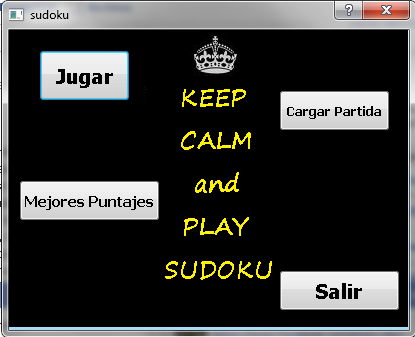
\includegraphics[width=.70\textwidth]{inicio.png}
\end{center}
El primer proyecto a presentar fue un juego llamado sudoku creado en Qt.
Sudoku es un pasatiempo que se publicó por primera vez a finales de la década de 1970 y se popularizó en Japón en 1986, dándose a conocer en el ámbito internacional en 2005 cuando numerosos periódicos empezaron a publicarlo en su sección de pasatiempos. 1 El objetivo del sudoku es rellenar una cuadrícula de 81 celdas  dividida en subcuadrículas de 9 (también llamadas "bloque") con las cifras del 1 al 9 partiendo de algunos números ya dispuestos en algunas de las celdas. Aunque se podrían usar colores, letras, figuras, se conviene en usar números para mayor claridad, lo que importa, es que sean nueve elementos diferenciados, que no se deben repetir en una misma fila, columna o subcuadrícula. Un sudoku está bien planteado si la solución es única. La solución de un sudoku siempre es un cuadrado latino, aunque el recíproco en general no es cierto ya que el sudoku establece la restricción añadida de que no se puede repetir un mismo número en una región.

\newpage
\begin{center}
\title{MANUAL DE USUARIO}\maketitle
\end{center}
\subsection*{¿Como se juega?}
El sudoku se presenta normalmente como una tabla de 81, compuesta por subtablas de 9 denominadas bloques".
Algunas celdas ya contienen números, conocidos como "números dados" o "pistas".
 El objetivo es rellenar las celdas vacías, con un número en cada una de ellas, de tal forma que cada columna, fila y  bloque contenga los números 1–9 sólo una vez.\\


\begin{center}
\section{¿Ques es una fila en el Sudoku?}
\end{center}
\begin{center}
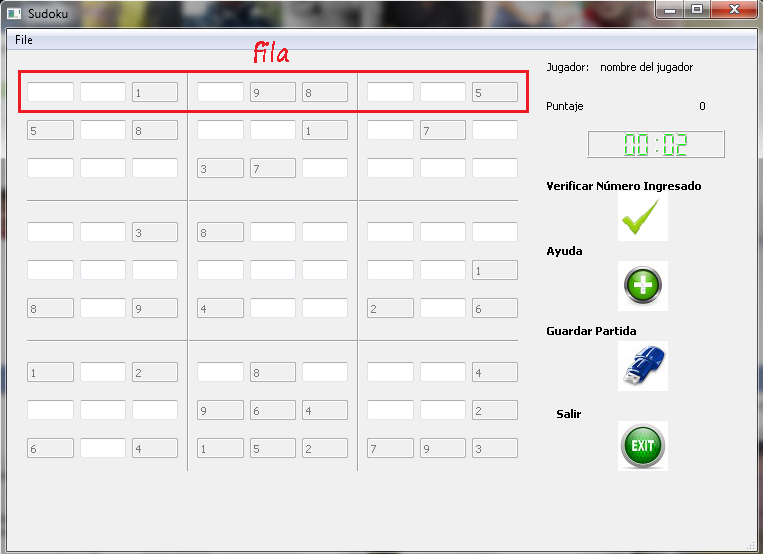
\includegraphics[width=12cm]{fila1.png}
\end{center}
En una Fila no podrá haber números repetidos\\

\begin{center}
\section{¿Ques es una Columna en el Sudoku?}
\end{center}
\begin{center}
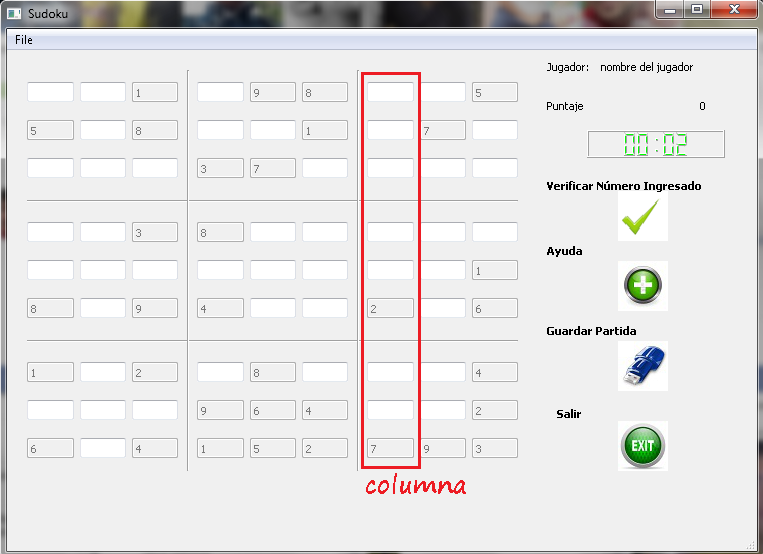
\includegraphics[width=12cm]{columna1.png}
\end{center}
En una Columna no podrá haber números repetidos\\

\begin{center}
\section{¿Ques es un Bloque en el Sudoku?}
\end{center}
\begin{center}
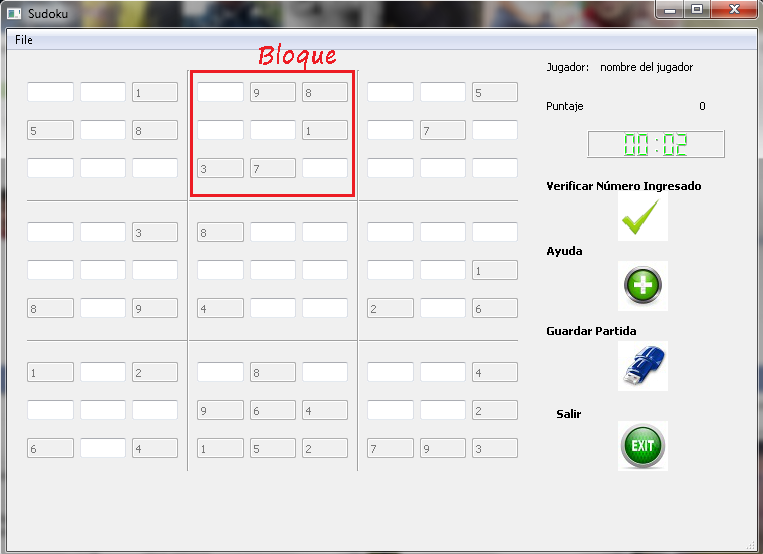
\includegraphics[width=12cm]{bloque1.png}
\end{center}
En un Bloque no podrá haber números repetidos\\

\begin{center}
\section{¿Como jugar en la aplicación?}
\end{center}
\begin{center}
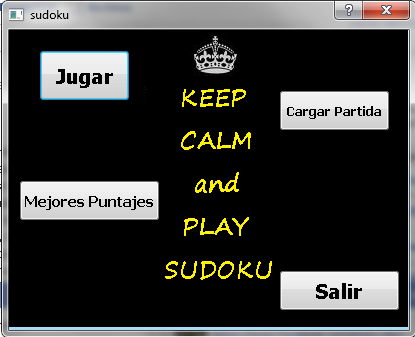
\includegraphics[width=12cm]{inicio.png}
\end{center}
Tenemos cuatro opciones si le damos clic en:\\
JUGAR aparecerá una nueva pantalla para seleccionar la dificultad y poner un nombre de jugador\\
CARGAR PARTIDA se cargara una partida guardada anteriormente\\
MEJORES PUNTAJES aparecerá una lista de los 5 mejores puntajes\\
SALIR para cerrar la aplicación\\


\begin{center}
\section{Cargar juego guardado}
\end{center}
\begin{center}
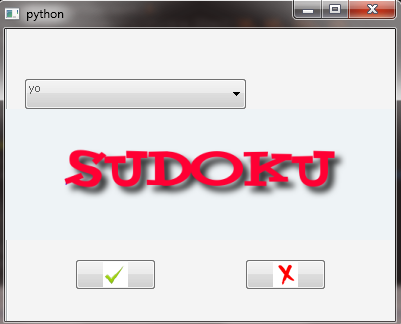
\includegraphics[width=12cm]{guardarpa.png}
\end{center}
Aqui podemos seleccionar una partida guardada anteriormente \\
si esta de acuerdo le da en el icono "VISTO" y nos aparecerá el juego\\ 
Si quiere salir debe dar clic en la "X" \\


\begin{center}
\section{Ventana de dificultad}
\end{center}
\begin{center}
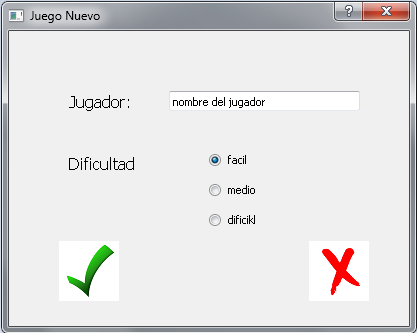
\includegraphics[width=12cm]{nombre_jug1.png}
\end{center}
Aqui podemos seleccionar un  nombre y también seleccionar una dificultad para el juego\\
si esta de acuerdo le da en el icono "VISTO" y nos aparecerá el juego \\
Si quiere regresar le da clic en la "X" \\


\begin{center}
\section{Inicio sudoku}
\end{center}
\begin{center}
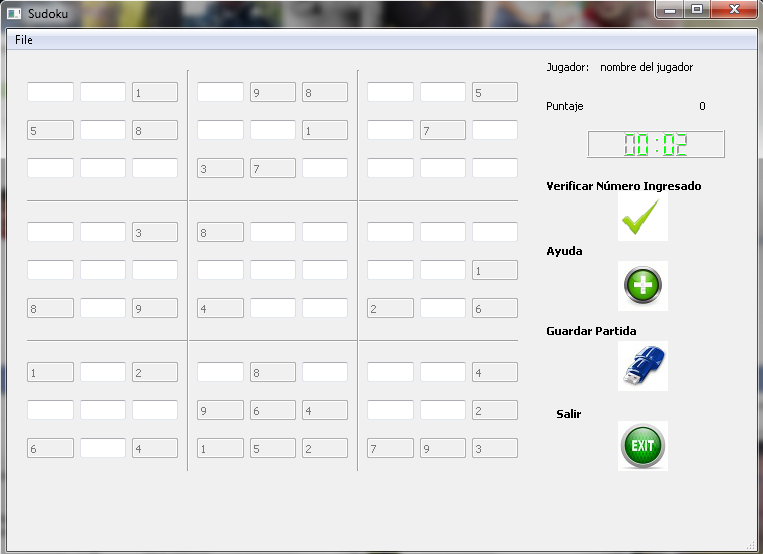
\includegraphics[width=12cm]{sudoku_ini1.png}
\end{center}
Aqui tenemos 4 opciones:\\
VERIFICAR FICHA INGRESADA\\
AYUDA\\
GUARDAR PARTIDA\\
SALIR\\


\begin{center}
\section{Ingreso de números}
\end{center}
\begin{center}
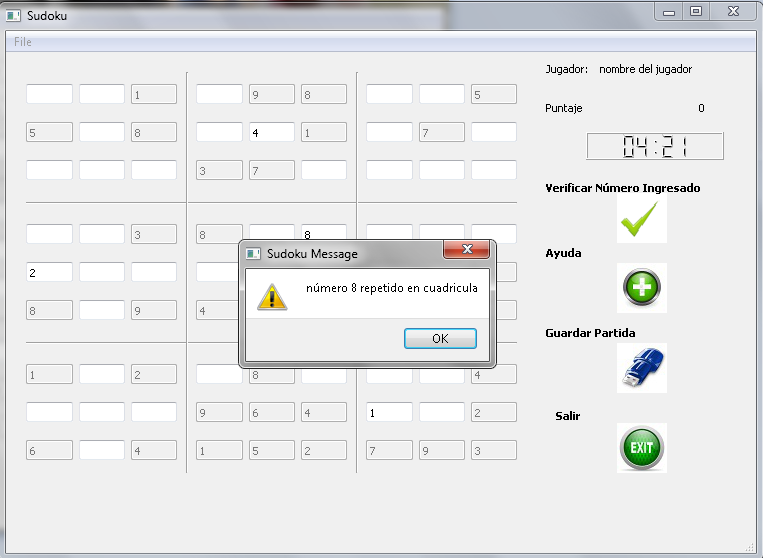
\includegraphics[width=12cm]{num_incorrecto1.png}
\end{center}
Aqui tenemos 4 opciones:\\
 Si da clic en VERIFICAR FICHA INGRESADA si esta correcta la aplicación no le dirá nada pero si esta incorrecta la aplicación le
botará una ventana emergente indicándole si ese número esta repetido en la fila,columna o bloque
Si da clic en AYUDA inmediatamente le aparecera un nuevo número en el tablero

\begin{center}
\section{Guardar partidas}
\end{center}
\begin{center}
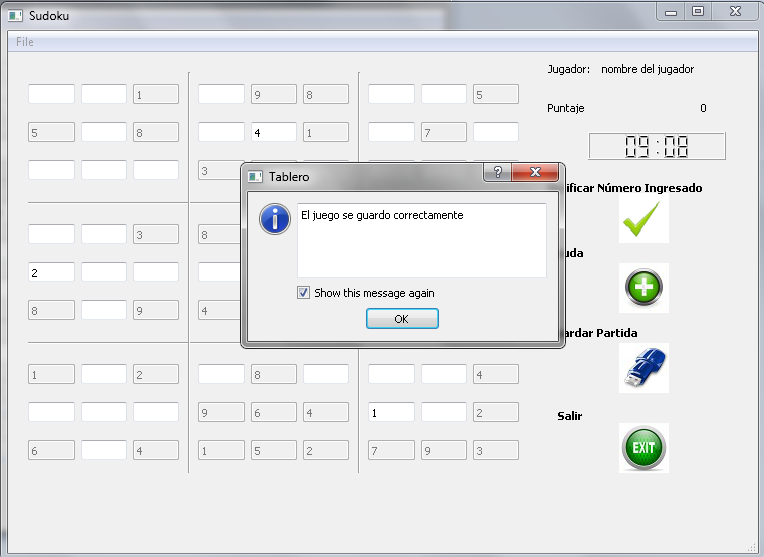
\includegraphics[width=12cm]{partida_guardada1.png}
\end{center}
Aqui tenemos 4 opciones:\\
Si da clic en GUARDAR PARTIDA automáticamente se guardara su partida y saldrá una ventana emergente indicandole que se guardo correctamente su partida\\
Si da clic en SALIR la aplicación se cerrara \\

\begin{center}
\section{terminar juego}
\end{center}
\begin{center}
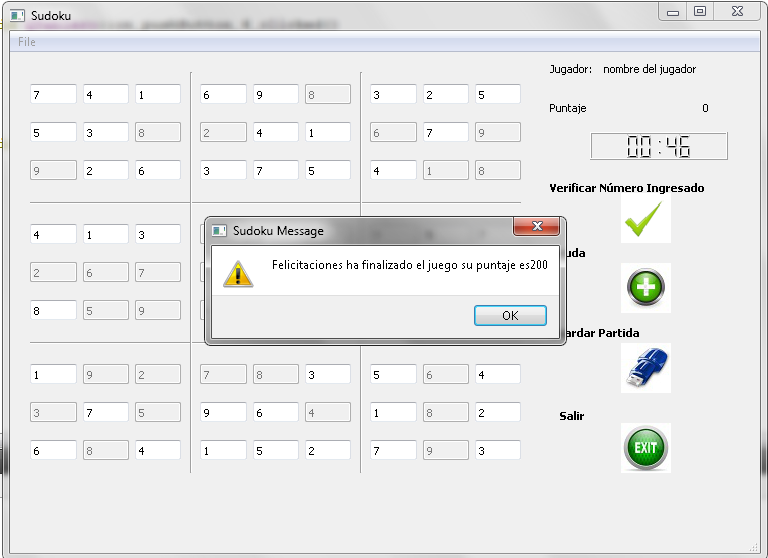
\includegraphics[width=12cm]{felicitaciones1.png}
\end{center}
Aqui tenemos 4 opciones:\\
Una vez ingresado todos los números y si estan correctos le aparecera una pantalla felicitándole y mostrándole su puntaje \\




\begin{center}
\section{CONCLUSIONES}
\end{center}

Manejar el lenguaje Qt fue una gran experiencia ya que mejore mis habilidades al programar y conoci nuevos comandos y una nueva forma de hacer una interfaz grafica y enlazar eventos a diferentes objetos de la aplicación,  este lenguaje en cuanto a codificación contiene un gran parecido a C++ y tambien un poco a java, se trabajo en Qt Creator la cual nos facilito mucho el aprendizaje de este lenguaje 
Ya que era similar a lenguajes de programación que anteriormente habiasmos utilizado no se nos dificulto mucho la realización del programa, pero si tuvimos un poco de inconvenientes al momento de crear eventos pero  inventigando pudimos solucionar todos nuestros problemas.
Qt es un lenguaje fácil de aprender  y muy recomendado para realizar programas sean estos pequeños juegos o programas más complejos.


\chapter{PHYTON}
\begin{center}
\title{\Large{PySudoku}}\maketitle

\includegraphics[width=.70\textwidth]{suini.jpg}
\end{center}

Nuestra segundo proyecto a presentar fue de hacer otra vez el sudoku pero esta vez  en una combinación de lenguajes  phyton y Qt (PyQt).
El proyecto consistía en hacer el mismo juego que lo habíamos hecho anteriormente en Qt, pero ahora en un lenguaje diferente, ya que es un lenguaje de programación multiparadigma, ya que soporta orientación a objetos, programación imperativa y, en menor medida, programación funcional. Es un lenguaje interpretado, usa tipiado dinámico y es multiplataforma.
\newpage
\begin{center}
\title{MANUAL DE USUARIO}\maketitle
\end{center}
\subsection*{¿Como se juega?}
El sudoku se presenta normalmente como una tabla de 81, compuesta por subtablas de 9 denominadas bloques".
Algunas celdas ya contienen números, conocidos como "números dados" o "pistas".
 El objetivo es rellenar las celdas vacías, con un número en cada una de ellas, de tal forma que cada columna, fila y  bloque contenga los números 1–9 sólo una vez.\\


\begin{center}
\section{¿Ques es una fila en el Sudoku?}
\end{center}
\begin{center}
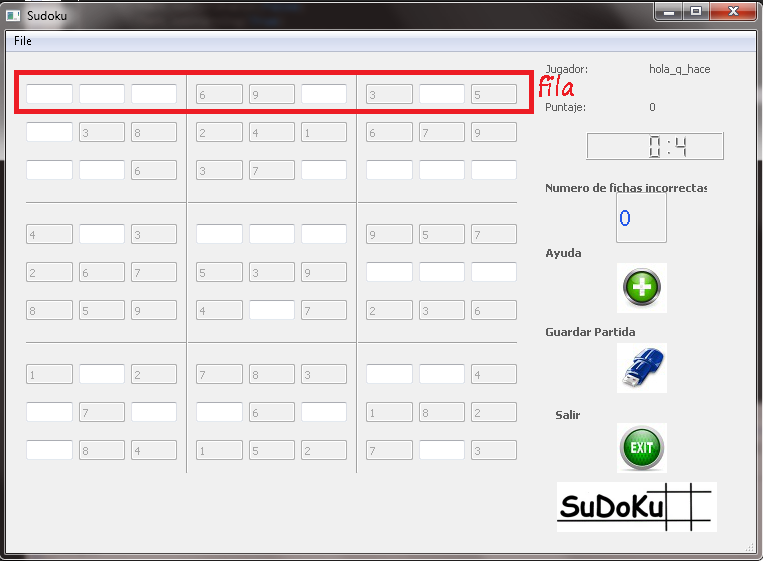
\includegraphics[width=12cm]{fila.png}
\end{center}
En una Fila no podrá haber números repetidos\\

\begin{center}
\section{¿Ques es una Columna en el Sudoku?}
\end{center}
\begin{center}
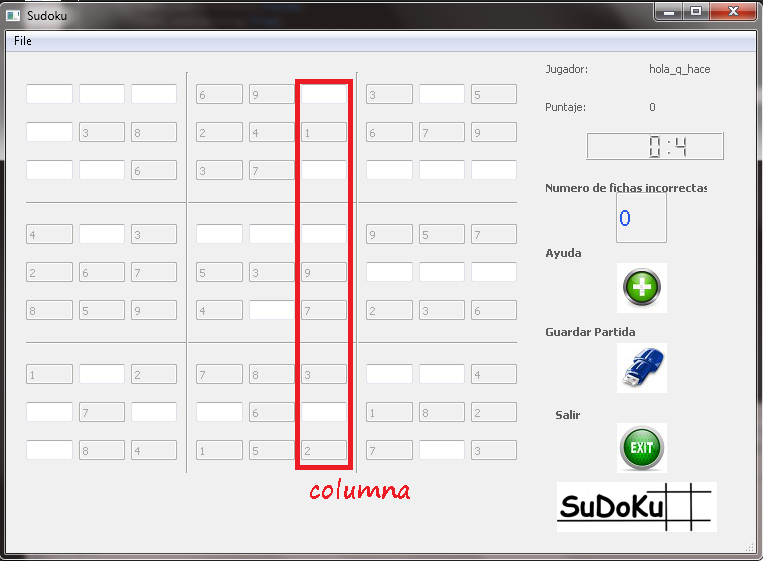
\includegraphics[width=12cm]{columna.png}
\end{center}
En una Columna no podrá haber números repetidos\\

\begin{center}
\section{¿Ques es un Bloque en el Sudoku?}
\end{center}
\begin{center}
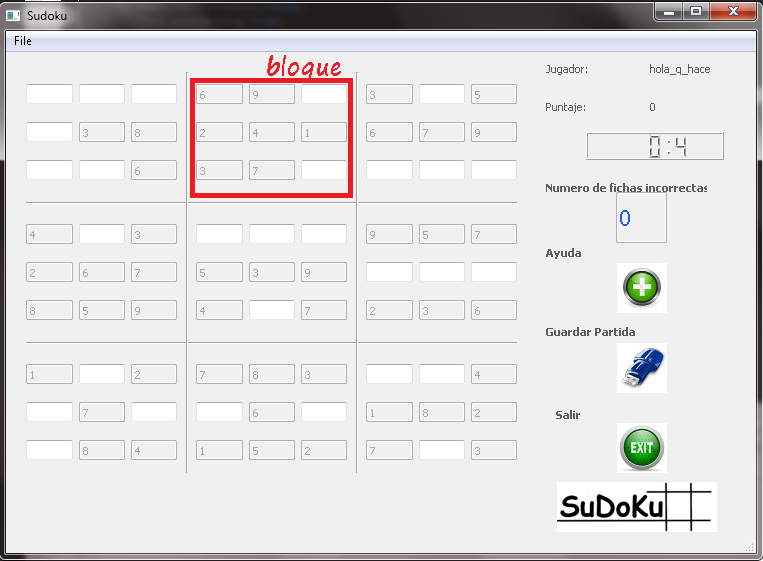
\includegraphics[width=12cm]{bloque.png}
\end{center}
En un Bloque no podrá haber números repetidos\\

\begin{center}
\section{¿Como jugar en la aplicación?}
\end{center}
\begin{center}
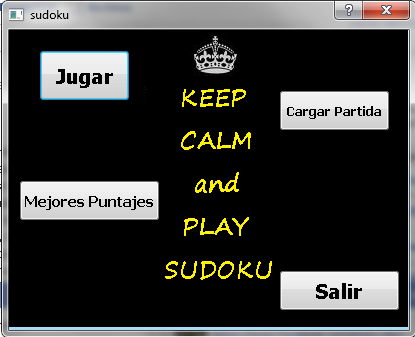
\includegraphics[width=12cm]{inicio.png}
\end{center}
Tenemos cuatro opciones si le damos clic en:\\
JUGAR aparecerá una nueva pantalla para seleccionar la dificultad y poner un nombre de jugador\\
CARGAR PARTIDA se cargara una partida guardada anteriormente\\
MEJORES PUNTAJES aparecerá una lista de los 5 mejores puntajes\\
SALIR para cerrar la aplicación\\


\begin{center}
\section{Cargar juego guardado}
\end{center}
\begin{center}
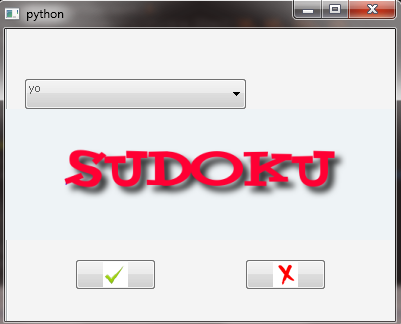
\includegraphics[width=12cm]{guardarpa.png}
\end{center}
Aqui podemos seleccionar una partida guardada anteriormente \\
si esta de acuerdo le da en el icono "VISTO" y nos aparecerá el juego\\ 
Si quiere salir debe dar clic en la "X" \\


\begin{center}
\section{Ventana de dificultad}
\end{center}
\begin{center}
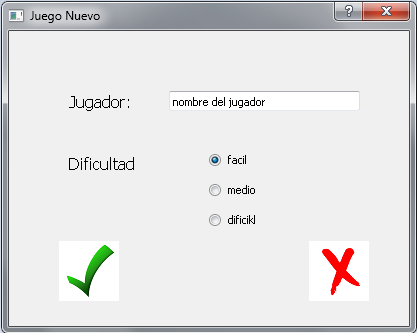
\includegraphics[width=12cm]{nombre_jug.png}
\end{center}
Aqui podemos seleccionar un  nombre y también seleccionar una dificultad para el juego\\
si esta de acuerdo le da en el icono "VISTO" y nos aparecerá el juego \\
Si quiere regresar le da clic en la "X" \\


\begin{center}
\section{Inicio sudoku}
\end{center}
\begin{center}
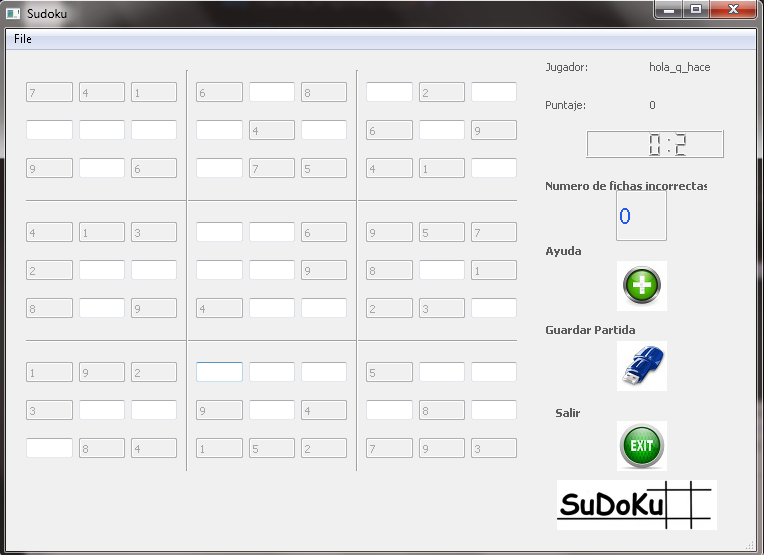
\includegraphics[width=12cm]{sudoku_ini.png}
\end{center}
Aqui tenemos 4 opciones:\\
MUESTRA CUANTAS VECES HEMOS INGRESADO UNA FICHA INCORRECTA\\
AYUDA\\
GUARDAR PARTIDA\\
SALIR\\


\begin{center}
\section{Ingreso de números}
\end{center}
\begin{center}
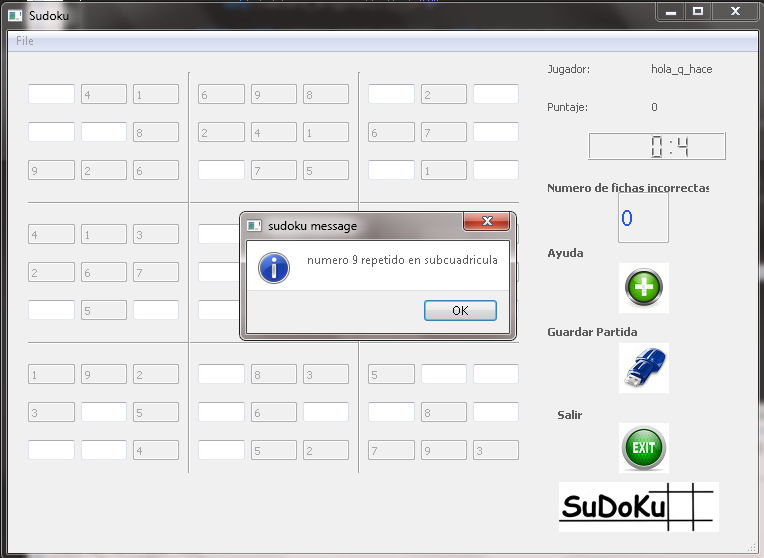
\includegraphics[width=12cm]{num_incorrecto.png}
\end{center}
Aqui tenemos 4 opciones:\\
Si da clic en AYUDA inmediatamente le aparecera un nuevo número en el tablero\\

\begin{center}
\section{Guardar partidas}
\end{center}
\begin{center}
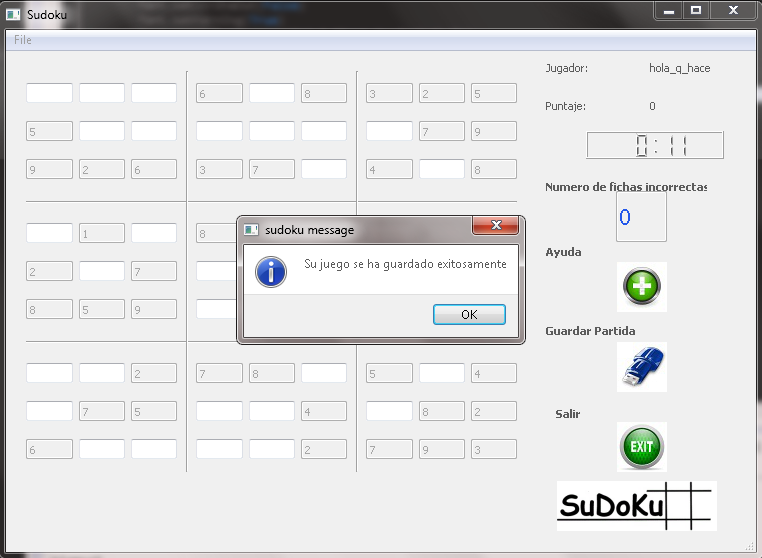
\includegraphics[width=12cm]{partida_guardada.png}
\end{center}
Aqui tenemos 4 opciones:\\
Si da clic en GUARDAR PARTIDA automáticamente se guardara su partida y saldrá una ventana emergente indicandole que se guardo correctamente su partida\\
Si da clic en SALIR la aplicación se cerrara \\

\begin{center}
\section{terminar juego}
\end{center}
\begin{center}
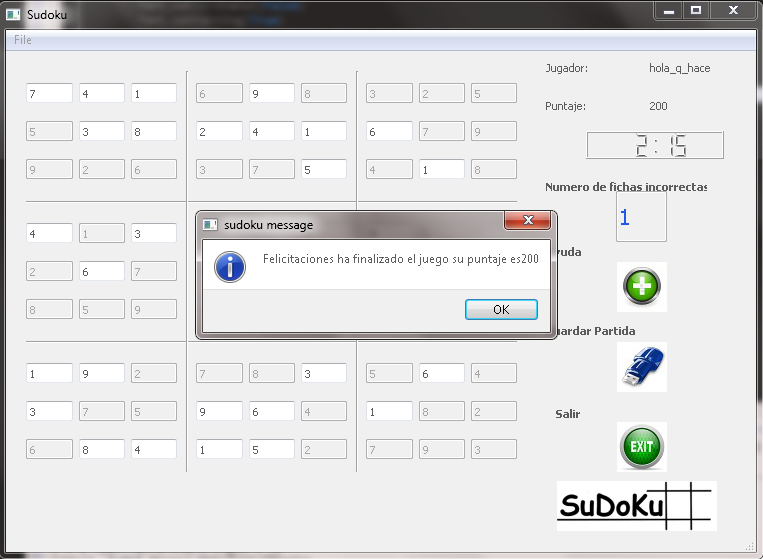
\includegraphics[width=10cm]{felicitaciones.png}
Aqui tenemos 4 opciones:\\
Una vez ingresado todos los números y si estan correctos le aparecera una pantalla felicitándole y mostrándole su puntaje 
\end{center}





\begin{center}
\title{CONCLUSIONES}\maketitle
\end{center}

La experiencia obtenida por este lenguaje  fue muy buena , como no habíamos trabajado antes con un lenguaje parecido se nos hizo un poco difícil comprenderlo y acostumbrarnos a el, por lo cual tuvimos que investigar en internet, este lenguaje tiene diferencias en cuanto a sintaxis de codificación, nuestro primer reto fue hacer la interfaz grafica del juego, pero investigando encontramos que PyQt tenía un convertidor de archivos .ui a .py, con esto pudimos solucionar el problema de crear la interfaz grafica y pudimos utilizar la que se había hecho en Qt.
la sintaxis para la creación de funciones y la implementación de eventos se hicieron más fáciles que en Qt, el desarrollo en este lenguaje al aprender a manejarlo nos daremos cuenta que no es complicado pero cuando todo es nuevo siempre tendremos dificultades.


\chapter{HASKELL}
\begin{center}
\title{\Large{Analizador Léxico}}\maketitle
\end{center}
El último lenguaje en aprender fue el haskell, en donde el proyecto ahora fue de crear un analizador léxico el cual consiste en que recibe como entrada el código fuente  y produce una salida compuesta de tokens (componentes léxicos) o símbolos




\begin{center}
\title{CONCLUSIONES}\maketitle
\end{center}

Este es un gran reto que todavía estamos tratando de vencer, ya que
este tipo de lenguaje funcional es muy diferente a los que normalmente
solemos aplicar, una ves terminado este proyecto implementaremos el
manual de usuario del mismo, para poder concluir con este pequeño
libro sobre las experiencias de usar todos estos lenguajes para nuestros
proyectos.


\newpage
\begin{center}
\title{ANEXOS}\maketitle
\end{center}
En esta sección anexaremos los codigos hecho en Pyton, Qt y haskell:\\
PHYTON\\
\href{https://github.com/Marvincin/ProyectoPython}{https://github.com/Marvincin/ProyectoPython}\\
HASKELL\\
\href{https://github.com/Marvincin/Haskell_Analizador}{https://github.com/Marvincin/HaskellAnalizador}\\
QT\\
\href{https://github.com/Marvincin/ProyectoCpp}{https://github.com/Marvincin/ProyectoCpp}\\

Estos son los repositorios de los proyectos realizados durante la materia

\begin{center}
\title{BIBLIOGRAFIAS}\maketitle
\end{center}

\href{http://lateral.netmanagers.com.ar/stories/BBS47.html}{http://lateral.netmanagers.com.ar/stories/BBS47.html}\\
\href{http://www.zonaqt.com/tutoriales}{http://www.zonaqt.com/tutoriales}\\
\href{http://aprendehaskell.es/content/Introduccion.html}{http://aprendehaskell.es/content/Introduccion.html}

\end{document}